\chapter{Materials}
\section{Stardard uniaxial materials}
\subsection{defElasticMaterial}
\noindent Construct an elastic uniaxial material
\begin{verbatim}
defElasticMaterial(mdlr,name,E)
\end{verbatim}
\vspace{-10pt}
{\color{grayLines} \rule{\linewidth}{0.25pt}}
\begin{center}
\begin{tabular}{lp{10cm}}
{\tt mdlr} & modeler name \\
{\tt name} & name identifying the material \\
{\tt E} & tangent in the stress-strain diagram (see figure \ref{Elastic}) \\
\end{tabular}
\end{center}
\paragraph{Example}
\begin{verbatim}
*
\end{verbatim}

\begin{figure}[h]
\centering
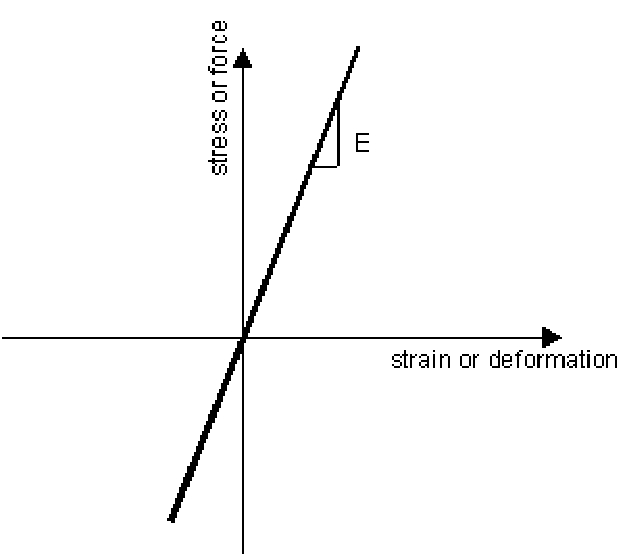
\includegraphics[width=60mm]{materials/figures/Elastic}
\caption{Elastic uniaxial material. Stress-strain diagram}\label{Elastic}
\end{figure}

\subsection{defElasticPPMaterial}
\noindent Construct an elastic perfectly-plastic uniaxial material
\begin{verbatim}
defElasticPPMaterial(mdlr,name,E,fyp,fyn)
\end{verbatim}
\vspace{-10pt}
{\color{grayLines} \rule{\linewidth}{0.25pt}}
\begin{center}
\begin{tabular}{lp{10cm}}
{\tt mdlr} & modeler name \\
{\tt name} & name identifying the material \\
{\tt E} & tangent in the elastic zone of the stress-strain diagram (see figure \ref{ElasticPP}) \\
{\tt fyp} & stress at which material reaches plastic state in tension (see figure \ref{ElasticPP}) \\
{\tt fyn} &  stress at which material reaches plastic state in compression (see figure \ref{ElasticPP}) \\
{\tt } &  \\
\end{tabular}
\end{center}
\paragraph{Example}
\begin{verbatim}
*
\end{verbatim}

\begin{figure}[h]
\centering
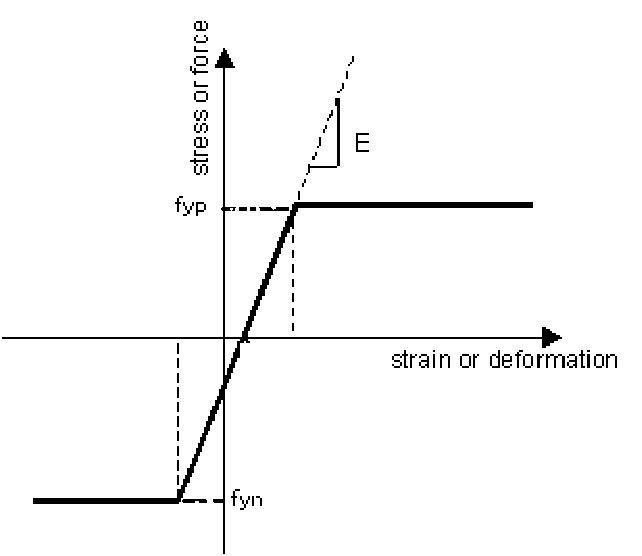
\includegraphics[width=60mm]{materials/figures/ElasticPP}
\caption{Elastic perfectly-plastic uniaxial material. Stress-strain diagram}\label{ElasticPP}
\end{figure}

\subsection{defElastNoTracMaterial}
\noindent Construct a uniaxial elastic-no tension material
\begin{verbatim}
defElastNoTracMaterial(mdlr,name,E)
\end{verbatim}
\vspace{-10pt}
{\color{grayLines} \rule{\linewidth}{0.25pt}}
\begin{center}
\begin{tabular}{lp{10cm}}
{\tt mdlr} & modeler name \\
{\tt name} & name identifying the material \\
{\tt E} & tangent in the elastic zone of the stress-strain diagram (see figure \ref{ENT}) \\
\end{tabular}
\end{center}
\paragraph{Example}
\begin{verbatim}
*
\end{verbatim}
\begin{figure}[h]
\centering
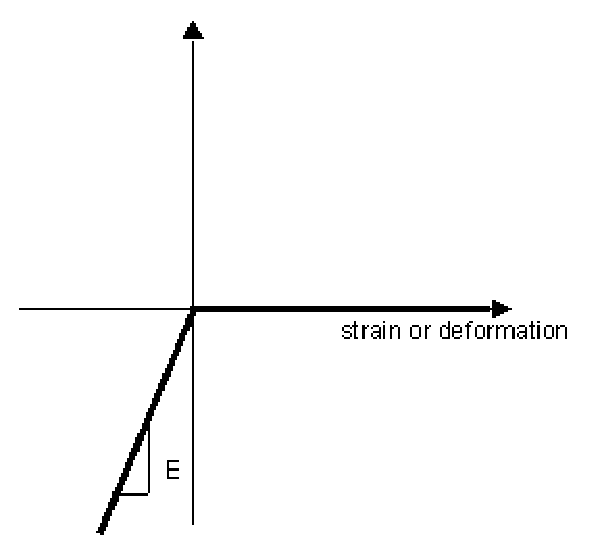
\includegraphics[width=50mm]{materials/figures/ENT}
\caption{Elastic-no tension material. Stress-strain diagram}\label{ENT}
\end{figure}

\section{Steel and reinforcing steel materials}
\subsection{defCableMaterial}
\noindent Construct a uniaxial bilinear prestressed material. The stress strain ranges from slack (large strain at zero stress) to taught (linear with modulus E).
\begin{verbatim}
defCableMaterial(mdlr,name,E,prestress,rho)
\end{verbatim}
\vspace{-10pt}
{\color{grayLines} \rule{\linewidth}{0.25pt}}
\begin{center}
\begin{tabular}{lp{10cm}}
{\tt mdlr} & modeler name \\
{\tt name} & name identifying the material \\
{\tt E} & Young modulus \\
{\tt prestress} & prestress \\
{\tt rho} & effective self weight (gravity component of weight per volume transverse to the cable) \\
\end{tabular}
\end{center}
\paragraph{Example}
\begin{verbatim}
*
\end{verbatim}


\subsection{defSteel01}
\noindent Construct a uniaxial bilinear steel material object with kinematic hardening% and optional isotropic hardening described by a non-linear evolution equation.
\begin{verbatim}
defSteel01(mdlr,name,E,fy,b)
\end{verbatim}
\vspace{-10pt}
{\color{grayLines} \rule{\linewidth}{0.25pt}}
\begin{center}
\begin{tabular}{lp{10cm}}
{\tt mdlr} & modeler name \\
{\tt name} & name identifying the material \\
{\tt E} & initial elastic tangent (see figure \ref{Steel01}) \\
{\tt fy} &  yield strength (see figure \ref{Steel01})\\
{\tt b} &  strain-hardening ratio: ratio between post-yield tangent and initial elastic tangent (see figure \ref{Steel01})\\
\end{tabular}
\end{center}
\paragraph{Example}
\begin{verbatim}
*
\end{verbatim}

\begin{figure}[h]
\centering
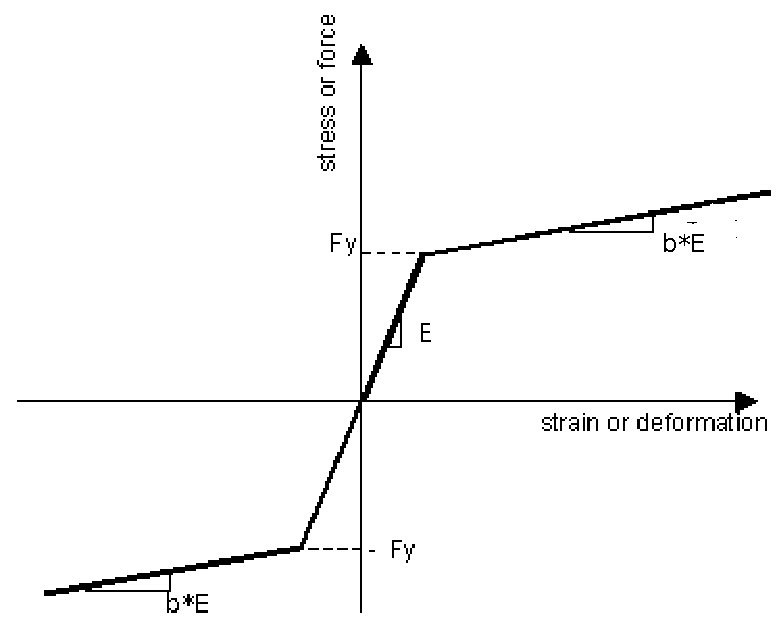
\includegraphics[width=60mm]{materials/figures/Steel01}
\caption{Steel001: uniaxial bilinear steel material with kinematic hardening. Stress-strain diagram}\label{Steel01}
\end{figure}


\subsection{defSteel02}
\noindent Construct a uniaxial Giuffre-Menegotto-Pinto steel material object with isotropic strain hardening
\begin{verbatim}
defSteel02(mdlr,name,E,fy,b,initialStress)
\end{verbatim}
\vspace{-10pt}
{\color{grayLines} \rule{\linewidth}{0.25pt}}
\begin{center}
\begin{tabular}{lp{10cm}}
{\tt mdlr} & modeler name \\
{\tt name} & name identifying the material \\
{\tt E} & initial elastic tangent (see figure \ref{Steel02}) \\
{\tt fy} &  yield strength (see figure \ref{Steel02})\\
{\tt b} &  strain-hardening ratio: ratio between post-yield tangent and initial elastic tangent)\\
{\tt initialStress} &  initial stress \\
\end{tabular}
\end{center}
\footnotesize{The transition from elastic to plastic branches  (see figure \ref{Steel02}) is controlled by parameters R0, R1, R2. The default values R0=15, R1=0.925 and R2=0.15}
\paragraph{Example}
\begin{verbatim}
*
\end{verbatim}

\begin{figure}[h]
\centering
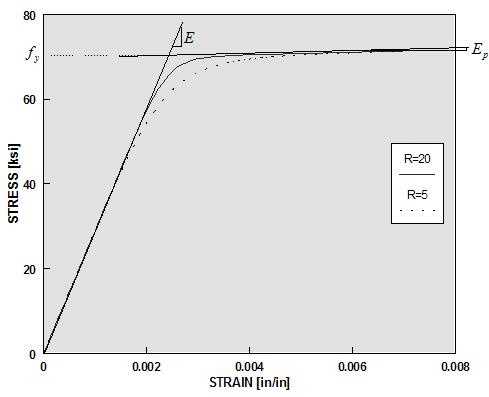
\includegraphics[width=60mm]{materials/figures/Steel02Monotonic}
\caption{Steel002: uniaxial bilinear steel material with isotropic strain hardening. Stress-strain diagram}\label{Steel02}
\end{figure}




\end{document}




\subsection{}
\noindent 
\begin{verbatim}

\end{verbatim}
\vspace{-10pt}
{\color{grayLines} \rule{\linewidth}{0.25pt}}
\begin{center}
\begin{tabular}{lp{10cm}}
{\tt } &  \\
{\tt } &  \\
{\tt } &  \\
\end{tabular}
\end{center}
\paragraph{Example}
\begin{verbatim}
*
\end{verbatim}

\begin{figure}[h]
\centering
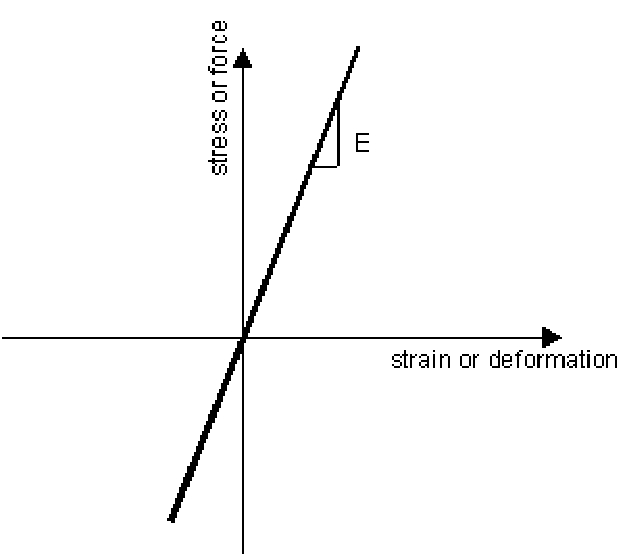
\includegraphics[width=60mm]{materials/figures/Elastic}
\caption{Elastic uniaxial material. Stress-strain diagram}\label{Elastic}
\end{figure}
